\documentclass{article}%You can define the type of paper here.
%%Useful packages that I commonly use.
\usepackage[numbers]{natbib}%Bibliography package (help at http://merkel.zoneo.net/Latex/natbib.php).
\usepackage{url}%Package to highlight url.
\usepackage{times}%Sets font to be times.
\usepackage{siunitx}
\usepackage{alltt}%Allows the use of verbatim (good for printing out code).
\usepackage{graphicx}%Used to import images.
\usepackage{amsmath, amssymb, amscd}%Contains the AMS expanded math symbols library.
\usepackage{algorithm, algorithmic} %pseudo-code
%%For those who want smaller margins, you can use this:
\usepackage[top=1in, bottom=1in, left=1in, right=1in]{geometry}


\begin{document}

%% Title =======================================================================

\title{Firn Densification Model}
\author{Cummings, Evan \and Davis, Tyler \and Brinkerhoff, Douglas}
\maketitle
\begin{center}

\includegraphics[width=0.45\textwidth]{images/logo.png}
\end{center}

\twocolumn


%% Introduction ================================================================
\section{Introduction}

The top layer of snow on a glacier or ice sheet increases in density as depth increases.  Several models have been created to simulate this process, some based on temperature and others based on enthalpy.  I have re-created these models with the finite-element software package FEniCS.

%% Temperature =================================================================
\section{Temperature Solution}

We begin with the standard heat-transport equation (Patterson, 2001

  $$
  \rho c_i \frac{\partial T}{\partial t} = 
    k_i \frac{\partial^2 T}{\partial z^2} +
    \left( \frac{dk}{dt} - \rho c_i w \right) \frac{\partial T}{\partial z}
  $$
with heat sources from the deformation of ice ommitted, $\rho$ density, $c_i$ heat capacity, $k_i$ thermal conductivity, $w$ vertical velocity, and $T$ temperature of firn.  To solve the total derivative $dk/dt$ we must apply the chain rule
  $$
  \frac{dk_i}{dz} = 
  \frac{\partial k_i}{\partial \rho} \frac{\partial \rho}{\partial z} + 
  \frac{\partial k_i}{\partial T} \frac{\partial T}{\partial z}.
  $$
The thermal conductiviy of ice is defined by Arthern et. al, 1998 as
  $$k_i = 2.1 \left(\frac{\rho}{\rho_i}\right)^2,$$
and gives
  $$
  \frac{\partial k_i}{\partial \rho} = 
    4.2 \frac{\rho}{\rho_i^2}
  $$
and
  $$
  \frac{\partial k_i}{\partial T} = 
    \frac{4.2}{\rho_i^2} \left( \frac{\partial \rho}{\partial T} \right).
  $$
Patterson, 2001 defined $\rho$ in terms of $T$ and from this can be derived
  $$
  \frac{\partial \rho}{\partial T} = 
    \SI{5.6e-2} \exp ((\SI{-5.7e-3})T).
  $$
The vertical velocity of ice, $w$, is directly proportional to the accumulation, $b$,
  $$
  w = -\frac{b}{\rho}
  $$
with $b$ in units of $kg\ m^{-2}\ s^{-1}$.  The densification process is defined with the material derivative
  $$\frac{d \rho}{dt} = \frac{\partial \rho}{\partial t} + 
    w\frac{\partial \rho}{\partial z}.$$
Arthern et. al, 2010 described the total derivative with the formula  
  $$
  \frac{d \rho}{dt} = 
  \begin{cases}
   c_0(\rho_i - \rho), &\rho <= 550\ kg\ m^{-3}\\
   c_1(\rho_i - \rho), &\rho > 550\ kg\ m^{-3}
  \end{cases}$$
Zwally and Li, 2002 defined the multiplying constant $c$ with an arrhenius-type relation
  $$
  c_0 = c_1 = 
  b \rho_i / \rho_w \beta(T)K_{0G}(T)\exp \left( -\frac{E(T)}{RT} \right),
  $$
with $K_{0G}(T) \exp(-E(T)/(RT)) = 8.36T^{-2.061}$, and $\beta(T)$ a smoothing function to match a desired density rate.  Arthern et. al 2010 developed a semi-empirical formula by coupling the rate equations for Nabarro-Herring creep and normal grain-growth : 
  $$
  \begin{cases}
    c_0 = M_0 bg\frac{k_{c0}}{k_g}\exp\left(-\frac{E_c}{RT} + 
          \frac{E_g}{RT_{avg}}\right)\\
    c_1 = M_1 bg\frac{k_{c1}}{k_g}\exp\left(-\frac{E_c}{RT} + 
          \frac{E_g}{RT_{avg}}\right)
  \end{cases},
  $$
with the creep coefficients defined as
  $$
  \begin{cases}
    k_{c0} = \SI{9.2e-9} m^3\ s\ kg^{-1} \\
    k_{c1} = \SI{3.7e-9} m^3\ s\ kg^{-1}  
  \end{cases}
  $$
and $M$ defined by Ligtenberg et. al 2011 to better fit with observed densification rates in higher-temperature environments :
  $$
  \begin{cases}
    M_0 = 2.366 - 0.293\ln(b*\SI{1e3})\\
    M_1 = 1.435 - 0.151\ln(b*\SI{1e3})
  \end{cases}.
  $$
Ligtenberg et. al 2011 developed a firn surface density expression from data :
  $$ \rho_s = -151.94 + 1.4266(73.6 + 1.06T_s + 0.0669A + 4.77V_a).$$


%% Enthalpy ====================================================================
\section{Enthalpy Solution}

As stated in Aschwanden et. al 2012, we take 'enthalpy' to be synonymous with 'internal energy' due to the exclusion of work done with changing volume.  The equation used here is the shallow-enthalpy :
	$$
  \rho \frac{\partial H}{\partial t} = \frac{\partial}{\partial z} 
    \left( 
      \begin{Bmatrix}
        K_i(H), &\text{Temperate}\\
        K_0, &\text{Cold}
      \end{Bmatrix}
      \frac{\partial H}{\partial z} 
    \right) + w \rho \frac{\partial H}{\partial z}.
  $$
Strain heating has been neglected and the advective term $w \rho\ \partial H / \partial z$ has been added.  The coefficient for temperate ice is 
  $$K_i(H) = \frac{k_i}{c_i}.$$
The coefficient for cold ice is
  $$K_0 = \frac{1}{10}K_i(H).$$
Temperate firn is defined as firn with $H > H_s$ and cold firn $H <= H_s$, with
  $$H_s = \int_{T_0}^{T_m}{c_i(T)}dT$$ 
where $T_m = 273.15$ K and $T_0 = 0.0$ K.  The enthalpy can be found with a constant heat capacity of $2009$ J kg$^{-1}$ K$^{-1}$ with the linear equation
  $$
  H = 
  \begin{cases}
    c_i(T - T_0), &\text{where } T <= T_m\\
    c_i(T_w - T_0) + \omega L_f,  &\text{where } T > T_m
  \end{cases}
  $$
where $L_f$ is the latent heat of fusion and $\omega$ represents the water content percentage of firn and is given by
  $$\omega L_f = H - c_i(T_w - T_0).$$
It is conveinent to find the temperature :
  $$T = \frac{H}{c}.$$
The density equations remain the same as the temperature solution.
The surface density can be described as : 
  $$\rho_s^{n+1} = \rho_s^{n} d_p + \rho_s^{n-1} (1 - d_p),$$
where
  $$\rho_s^{n} = \rho_s^{n-1} + d\omega_s \rho_b,$$
  $$d\omega_s = \omega_s^{n} - \omega_s^{n-1},$$ 
  $$d_p = \frac{d}{l_s},$$
  $$d = w_sdt,$$
$l_s$ is the length of the surface node, and
  $$
  \rho_b = 
  \begin{cases}
    300\ \text{kg m}^{-3},  &T > T_w\\
    1000\ \text{kg m}^{-3}, &T <= T_w
  \end{cases}.
  $$


%% Method ======================================================================
\section{Finite Element Method}

This section will focus on the enthalpy solution; solving these equations with FENicS is done with Galerkin's method which requires finding the weak formulation :
  $$
    0 =
    \int_{\Omega} 
      \begin{Bmatrix}
        K_i(H)\\
        K_0
      \end{Bmatrix}
      \nabla^2 H \psi\ d \Omega 
    + \int_{\Omega}w \rho \nabla H \psi\ d \Omega
  $$
  $$
    - \int_{\Omega} {\rho \frac{\partial H}{\partial t}} \psi\ d \Omega.
  $$
Here we have integrated over the entire domain, $\Omega$, and multiplied by a test function $\psi$.  After integrating the diffusive term by parts this becomes
  $$
    f_H =
    - \int_{\Omega} 
        \begin{Bmatrix}
          K_i(H)\\
          K_0
        \end{Bmatrix}
        \nabla H \nabla \psi\ d \Omega 
    + \int_{\Omega}w \rho \nabla H \psi\ d \Omega
  $$
  $$
    - \int_{\Omega} {\rho \frac{\partial H}{\partial t}} \psi\ d \Omega.
  $$
We can descritize the enthalpy timee-differential with the second-order accurate backward-difference formula
  $$\frac{\partial H}{\partial t} = \frac{H^{k-2} - 4H^{k-1} + 3H}{2dt},$$
with superscripts referring to time index.  This equation can be represented in FENicS as :
\small
\begin{alltt}
f_H = (rho*(H_2 - 4*H_1 + 3*H)/(2*dt)*psi 
      + k/c*Kcoef*inner(grad(H), grad(psi))
      + rho*w*grad(H)*psi)*dx
\end{alltt}
\normalsize
The variable \texttt{Kcoef} is a coefficient vector which will be updated dynamically depending on the temperature of firn (either $1.0$ or $0.1$).

The weak form for density is found similarly :
  $$
  f_{\rho} = 
    \int_{\Omega} \frac{\partial \rho}{\partial t}\phi\ d \Omega + 
    \int_{\Omega} w\nabla \rho \phi\ d \Omega -
    \int_{\Omega}\frac{d \rho}{dt}\phi\ d \Omega.
  $$
With the partial-time-differential of density defined indentically to the enthalpy equation, this can be represented in FENicS with the Arthern et. all 2010 densification equation as :
\small
\begin{alltt}
c      = b*g*rhoCoef/kg * 
         exp(-Ec/(R*T) + Eg/(R*Tavg))
drhodt = c*(rhoi - rho)
f_rho  = ((rho_2 - 4*rho_1 + 3*rho)/(2*dt) 
         - drhodt + w*grad(rho))*phi*dx 
\end{alltt}
\normalsize
The variable \texttt{rhoCoef} is another dynamically-updated-coefficient vector and is either $k_{c0}$ or $k_{c1}$ depending upon the density at the node.

We can define the function space for the entire non-linear problem as 
  $$
    U = \Omega \times \Omega,
  $$
with corresponding trial and test functions respectively defined as
  $$
    v, u \subset U.
  $$
The test functions for each function can now be described as
  $$
    \psi, \phi \subset u.
  $$
In FENicS these spaces can be defined by this :
\small
\begin{alltt}
V         = FunctionSpace(mesh, 'Lagrange', 1)
MV        = V*V
h         = Function(MV)
H,rho     = split(h)    
dh        = TrialFunction(MV)
dH, drho  = split(dh)
j         = TestFunction(MV)
psi, phi  = split(j)
\end{alltt}
\normalsize

We define the function as 
  $$
    f = f_H + f_{\rho}.
  $$
Solving this system can be accomplished by \emph{Newton's Method} and requires the derivation of the Jacobian :
  $$
    J = \frac{\partial f}{\partial U}
  $$
In FENicS this becomes :
\small
\begin{alltt}
f  = f_H + f_rho
J  = derivative(f, h, dh)
\end{alltt}
\normalsize

Now all that is left is to iterate through time and call the \texttt{solve} method :
\small
\begin{alltt}
solve(f == 0, h, [Hbc, Dbc], J=J)
\end{alltt}
\normalsize

  $$l_{n+1} = l_n \frac{\rho_{ini}}{\rho}$$
  $$s_{n} = (z_s - z_b) \frac{s_{n-1} - z_b}{z_{s} - z_b} + w_s dt $$


%% Verification ================================================================
\section{Verification of Program}
Using the values given in the previous two sections results in these figures :
\begin{figure}[H]
	\centering
		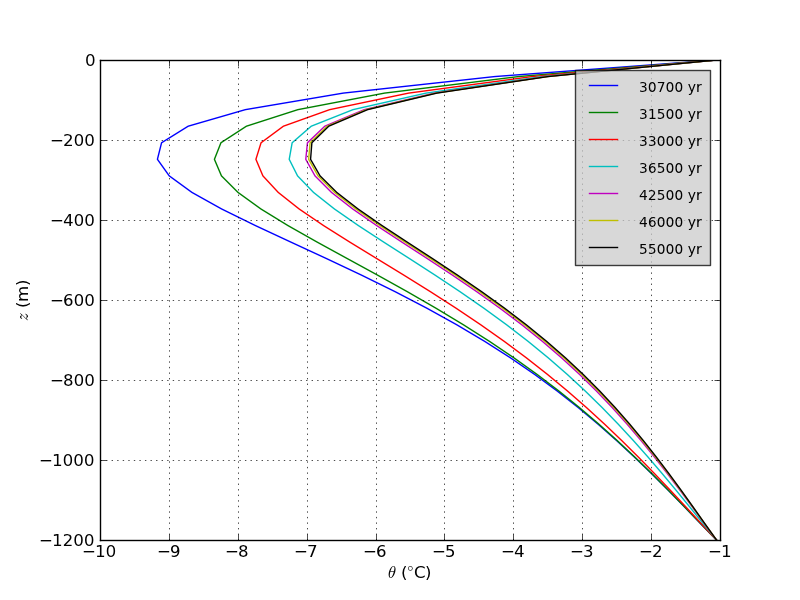
\includegraphics[width=0.42\textwidth]{images/60000yr_converge.png}
	\label{fig:500 year orbit}
	\caption{Temperature of Ice after Biasing the Temperature by $+15\ ^\circ C$}
\end{figure}


%% Interpretation ==============================================================
\section{Interpretation}


\end{document}
%%Compile with pdflatex file.tex



